\documentclass[12pt,twoside,a4paper]{article}
\setlength{\oddsidemargin}{-0.4mm} % 25 mm left margin
  \setlength{\evensidemargin}{\oddsidemargin}
  \setlength{\textwidth}{160mm}      % 30 mm right margin
  \setlength{\topmargin}{-5.4mm}     % 20 mm top margin
  \setlength{\headheight}{5mm}
  \setlength{\headsep}{5mm}
  \setlength{\footskip}{10mm}
  \setlength{\textheight}{237mm}     % 20 mm bottom margin
\usepackage{epsfig,authblk}
\usepackage{xcolor}
\usepackage[pdfpagelabels=false,pdfborder={0 0 0}]{hyperref}
\usepackage{graphicx}
\usepackage{listings}
\usepackage{titlesec}

\newcommand{\pname}{Resourceful}
\newcommand{\lnote}[1]{\textcolor{red}{[\textit{#1}]}} %notes
\newcommand*\aorder[1][\value{footnote}]{\footnotemark[#1]}
\renewcommand\Authsep{\hskip 1cm} \renewcommand\Authands{\hskip 1cm}

\titlespacing\section{0pt}{8pt plus 4pt minus 2pt}{3pt plus 2pt minus 2pt}
\titlespacing\subsection{0pt}{8pt plus 4pt minus 2pt}{3pt plus 2pt minus 2pt}
%\setlength{\textfloatsep}{8pt plus 1.0pt minus 2.0pt}

\colorlet{punct}{red!60!black}
\definecolor{background}{HTML}{EEEEEE}
\definecolor{delim}{RGB}{20,105,176}
\colorlet{numb}{magenta!60!black}

\lstdefinelanguage{json}{
    basicstyle=\normalfont\ttfamily,
    numberstyle=\scriptsize,
    stepnumber=1,
    numbersep=8pt,
    showstringspaces=false,
    breaklines=true,
    frame=lines,
    literate=
     *{0}{{{\color{numb}0}}}{1}
      {1}{{{\color{numb}1}}}{1}
      {2}{{{\color{numb}2}}}{1}
      {3}{{{\color{numb}3}}}{1}
      {4}{{{\color{numb}4}}}{1}
      {5}{{{\color{numb}5}}}{1}
      {6}{{{\color{numb}6}}}{1}
      {7}{{{\color{numb}7}}}{1}
      {8}{{{\color{numb}8}}}{1}
      {9}{{{\color{numb}9}}}{1}
      {:}{{{\color{punct}{:}}}}{1}
      {,}{{{\color{punct}{,}}}}{1}
      {\{}{{{\color{delim}{\{}}}}{1}
      {\}}{{{\color{delim}{\}}}}}{1}
      {[}{{{\color{delim}{[}}}}{1}
      {]}{{{\color{delim}{]}}}}{1},
}

\hypersetup{
    colorlinks=true,
    linkcolor=black,
    citecolor=black,
    filecolor=black,
    urlcolor=black,
}

\begin{document}
\lstdefinestyle{customc}{
  belowcaptionskip=1\baselineskip,
  frame=lines,
  breaklines=false,
  language=json,
  showstringspaces=false,
  basicstyle=\scriptsize\ttfamily,
}
%don't want date printed
\date{}

%make title bold and 14 pt font (Latex default is non-bold, 16 pt)
\title{\Large \bf \pname: fine-grained resource accounting\\for explaining service variability}

%for single author (just remove % characters)
\author{Lucian Carata\thanks{in alphabetical order}\aorder} \author{Oliver
Chick\aorder} \author{James Snee\aorder} \author{\authorcr{}Ripduman Sohan}
\author{Andrew Rice} \author{Andy Hopper} \affil{Computer Laboratory, University
of Cambridge, UK\\ \texttt{\{firstname.lastname\}@cl.cam.ac.uk}}

\maketitle

% Use the following at camera-ready time to suppress page numbers.
% Comment it out when you first submit the paper for review.
%\thispagestyle{empty}
\setcounter{page}{3}


\subsection*{Abstract}
Increasing server utilization in modern datacenters also increases the
likelihood of contention on physical resources and unexpected behavior due to
side-effects from interfering applications. Existing resource accounting
mechanisms are too coarse-grained for allowing services to track the causes of
such variations in their execution. We make the case for measuring resource
consumption at system-call level and outline the design of \emph{Resourceful}, a
system that offers applications the ability of querying this data at runtime
with low overhead, accounting for costs incurred both synchronously and
asynchronously after a given call.

\section{Introduction} 
Running multiple services on the same physical host, multiplexed over a pool of
shared resources, is a common method for increasing machine utilization. This is
typically achieved through operating system process separation, containerization
or hypervisor-based virtualization. However, depending on the workloads
of the collocated services, the increase in utilization may also increase
contention on system resources. This translates into greater variability in
system behavior, and lower predictability in terms of performance and failure
rates \cite{dean2013}.

By design, the control planes managing hardware resources (the hypervisor and/or
the OS kernel) are viewed as black boxes by any applications executing on top.
This means that there is no direct way for a single process to detect or query
whether its execution is affected by resource contention (e.g. cache trashing, IO
storms). Furthermore, it is difficult to diagnose and recover from side effects
of performance degradation caused by contention (e.g. fewer results returned, loss of
precision in timeout-based processing algorithms).

%Any system experiencing high contention on particular resources will show more
%variability in its behavior, becoming less predictable in terms of performance
%and failure rates \cite{?}. This is why resource consumption metrics like CPU,
%memory or IO are often used as a proxy for system behavior and health, in both
%human-driven and automated processes (e.g. by an engineer evaluating increased
%tail latency causes or a distributed scheduler making decisions about task
%migration).

%However, low resource usage is not desirable, either: there has been a constant
%push for increasing server utilization and reducing running costs in modern
%datacenters. Those are typically achieved through service aggregation, where
%multiplexing several applications on a single physical host is done either
%through hypervisor-based virtualization (VM's), lightweight virtualization
%(containers), or by running multiple services on the same OS, depending on the
%required level of isolation, SLAs, etc. %\lnote{In order to lower overheads, it
%% seems likely that lighter-weight OS-based virtualization solutions such as
%% containers will become more common.}

The fundamental step towards enabling applications to measure and react to periods of
resource contention during their execution is giving them the ability to query
detailed resource consumption data on the actions they perform. To this end, we
present \pname, a framework that provides configurable resource utilization
measurements at system call granularity to applications interested in monitoring
their footprint in the context of overall resource consumption.

%As more services will start sharing the same hardware resources, the importance
%of measuring and understanding both the causes and consequences of such
%variations in the properties of the system will increase. This justifies the
%need for gathering accurate resource accounting data \lnote{at the
%hypervisor/kernel level?}.
For actions performed completely in user space, applications can already be
instrumented to monitor their own execution. In contrast, once a system call is
made, they no longer have any control or visibility into what happens at kernel
level in terms of resource consumption. However, many applications end up
spending a significant percentage of their time in the
kernel~\cite{boyd2010analysis}.

It is possible to make coarse-grained measurements at this level in terms of
\textit{aggregate} resource consumption using existing profiling and monitoring
tools. For example, the Linux kernel provides mechanisms such as the
\texttt{getrusage()}\footnote{\url{http://www.gnu.org/software/libc/manual/html_node/Resource-Usage.html}} call, \texttt{perf}\footnote{\url{https://perf.wiki.kernel.org/index.php/Main_Page}}, and \texttt{ftrace}\footnote{\url{https://www.kernel.org/doc/Documentation/trace/ftrace.txt}}. Other tools such
as \texttt{iotop}\footnote{\url{http://guichaz.free.fr/iotop/}} or \texttt{netstat}\footnote{\url{http://linux.die.net/man/8/netstat}} use information exposed through
\texttt{$/$proc}, while DTrace \cite{dtrace} and SystemTap \cite{systap} allow the user to write scripts that can gather
similar data. However, current methods fall short in the following important
dimensions:

(i) \textbf{Accounting granularity and aggregation:} The mechanisms
above can only obtain system-wide or per-process statistics. Therefore, it is
difficult to understand the contribution of a particular process'
\textit{activity} towards total resource consumption. For example, if one
wishes to diagnose occasional high latency responses from a server, then
per-process aggregated data is of limited use. Instead, fine-grained information is
needed, such as per system call data aggregated only over the lifetime of the
request-response cycle. Existing tools that can track individual function calls,
such as \texttt{ftrace}, are often limited to debugging scenarios because of the overheads
they introduce.

(ii) \textbf{Accounting for resources consumed asynchronously:} not all the
effects of a given system call occur during its execution. A very simple example
here is a process writing data to disk: while the application makes multiple
calls to \texttt{write()} on a particular file descriptor, there may be no
immediate I/O activity on disk because of the kernel's use of a buffer cache.
The actual submission to hardware will occur asynchronously, depending on the
I/O scheduler, the expiration of a flushing interval, or on an explicit call to
\texttt{fsync}. Simply recording resource consumption metrics before and after a
\texttt{write} call will not capture its full cost. In order to fully explain
shared resource usage, one needs to take into account asynchronous effects and
assign the costs of running them to original causes. There are no existing tools
supporting this type of investigation.

(iii) \textbf{Online analysis and feedback:} with the exception of
\texttt{getrusage()}, most kernel-level resource accounting mechanisms available
are designed for debugging or offline analysis scenarios -- the final output is
a log that needs to be processed in order to extract relevant data. The
applications themselves never have access to this data while running, and
therefore cannot adapt in real time to other concurrent workloads. Instead,
applications are given the illusion of exclusive resource ownership.

The difficulty in providing the OS support for dealing with those issues can be
attributed to the high overhead that is typically introduced by fine grained
measurements and to the challenge of tracking causal dependencies between pieces
of code executed by the kernel. \pname{ }addresses these problems through
\emph{selective} kernel probing, informed by static binary and code analysis.

The main contributions of this paper are: 

\begin{itemize} 
\item Describing an architecture that allows applications to gather fine-grained
(system call level) resource consumption data, broken down per kernel subsystem,
with low overhead.
\item Presenting a method for automatically identifying kernel subsystem
boundaries and the minimal number of required instrumentation probe points,
using static analysis.
\item A framework for attributing resource consumption of asynchronous
tasks to the calls that triggered their execution.
\end{itemize}

Our current implementation focuses on gathering resource usage data from the
Linux kernel.  However, the overall design is general enough to allow for
implementation in hypervisors and extension to other codebases. 
% set up reasonable expectations:

In this paper, we show that it is possible to run a system tracking resource
consumption based on our design with reasonable overhead. Our initial experiments
consider accounting for socket accept/send/receive resource consumption in a
real application (lighttpd). A full investigation on the accuracy of the
recorded data remains as future work.


\section{\pname: System design} 
Fine-grained accounting is required in cases where developers need insights into the way applications behave or interact with each other: for example, one might want to understand the cost of a client request, either on a single host or over a distributed system; this implies being able to aggregate data at sub-process granularity (summing over the calls that were made to service that request). On high latency requests, there is a need of diagnosing causes: What is different from the low latency case? Were there unintended interactions between the server and other co-located applications? Where was most of the time spent?

The same fine-grained resource usage data can be used in improving user-level scheduling, or application coordination: applications could take such decisions based on the current state, for example by task-level coalescing of requests~\cite{dogar2014}, or could trade resources similar to auction frameworks~\cite{ShiAuction2014}. 

With these use cases in mind, \pname{ }is designed to give applications full
control over measuring resource consumption of system calls. The framework has
three main components: (i) \textit{measurement configuration:} this analyzes the
current kernel in order to identify a minimal set of instrumentation probe
points and subsystem boundaries (the level at which aggregation takes place),
guided by a user-provided configuration; (ii) \textit{a kernel module}
responsible for inserting these probes into the kernel and activating them when
applications request resource consumption data and (iii) \textit{a user-space
library} exposing an API that applications can use to express interest in the
resource consumption of particular system calls and to read the results after
the required information was gathered on the kernel side.

Each resource accounting result provides detailed metrics grouped by kernel
subsystem. For example, the data recorded for one system call would contain
total CPU cycles, wall clock time and memory costs, but these
values are further broken down for each functional subsystem touched during that call: total
CPU cycles spent in the Network subsystem, total cycles spent in VFS and
subsystem-specific metrics such as bytes sent/received, number of
retransmissions, IO queue size, disk writes. The application can select exactly
which of those metrics are recorded and can also perform custom aggregations
across multiple system calls.

By reporting resource consumption aggregated by subsystem, Resourceful provides
a more detailed view of what happens inside the kernel. For example, given a
socket \texttt{send()} operation, the application can view the breakdown
of latency and answer questions such as: Was most of the time spent in the
network stack? Was the packet delayed by the scheduler moving the task on a
different core?

\subsection{Kernel subsystem identification}

The Linux kernel has a modular structure of \emph{subsystems}, such as VFS,
logical filesystems, block devices. A complete list of these can be found in
the Linux Kernel Map.\footnote{\url{http://www.makelinux.net/kernel_map/}} \pname{ }uses this logical structure in identifying suitable probing points for
reporting the resource consumption on a per-subsystem basis.

%\lnote{(lc525): see par end} This differs from current approaches that typically fall
%into two categories: \textit{per-process} resource consumption, which lacks the
%resolution for determining the cause of bottlenecks and \textit{per-function}
%consumption, such as performed by ftrace. This has a high performance overhead
%(up to 3x in some situations), and produces lots of data requiring
%post-processing to extract usable information. 
%\lnote{(lc525): questionable whether we should have this here,
%we have mentioned before how we differ from others}

%Our approach allows us to give performance characteristics at a
%level whereby information can be used without post-processing, but with a high
%degree of granularity. Moreover, code paths changing subsystem is more rare than
%function calls, so we read counters less often, thereby achieving a lower
%overhead.

To identify subsystems, we perform inter-procedural static analysis of the
currently-running kernel. We start by finding all \texttt{call} instructions in
the kernel's binary, and determine the function symbols for both the callee and
the caller. Each function is then categorized into one of the subsystems in the
Linux Kernel Map, predominantly based on its source file location. We track the
function calls that are made from within one subsystem to another, and we
consider them to be part of the subsystem boundary.

\vspace{1em}
\lstset{style=customc, captionpos=b}
\begin{lstlisting}[caption={Sample configuration file defining a custom subsystem},label={lst:config}]
global {
  subsystem_whitelist: net_link_layer
}

subsystem net_link_layer {
  boundary:
    probe dev_queue_xmit {
      arg    : skb
      capture: {
        name: net_buf_enq,
        val : &skb->dev->qdisc
      }
    },
    probe qdisk_restart {
      arg    : dev
      capture: {
        name: net_buf_deq,
        val : &dev->qdisc
      }
    }
  metrics: cycles
  map_async: match(net_buf_deq, net_buf_enq)
}
\end{lstlisting}

Instrumentation probes are then inserted around the locations where such
boundary functions are called. Concretely, if the \texttt{sys\_socket} function
(from the Network subsystem) calls \texttt{kmalloc} (from the Memory subsystem),
we need to add probes surrounding the call site of \texttt{kmalloc} within
\texttt{sys\_socket}. Even if this means we could potentially be setting
numerous probes (a function such as kmalloc is called often), it is the only way
to avoid false positives: setting the probes inside \texttt{kmalloc} would mean
probing more often than necessary: any call to \texttt{kmalloc} would be probed,
even when it's not on a subsystem boundary (e.g any call to \texttt{kmalloc} from
within the Memory subsystem). Whilst inserting more probes has a higher startup
cost, there is no runtime cost of unused probes and there is no increase in code
size from inserting unused probes.

Besides the subsystems identified automatically this way, we allow users to
influence the process through configuration files such as the one presented in
Listing~\ref{lst:config}. Here, users can remove subsystems detected
automatically or add their own. The example shows how the network link layer
could be defined as a separate subsystem, generating probes for when packets are
enqueued or dequeued from device buffers.

So far, we have applied our analysis to the Linux kernel. However, this
approach can be extended to any codebase where modules are organized using a
directory-based structure.

% Todo fn pointers
% Can be done on any kernel, without the need for source or recompilation.

\subsection{Kernel accounting infrastructure}

Having identified the minimum number of probe points required for measuring per-subsystem
resource consumption, a kernel module has the job of inserting those probes at runtime.
For the Linux kernel, this can be achieved using kprobes.\footnote{\url{https://www.kernel.org/doc/Documentation/kprobes.txt}}

When triggered, each kprobe records a snapshot of resource consumption metrics according
to the subsystem in which the probed function resides. For gathering actual data, we
use existing kernel mechanisms such as \texttt{perf\_events} for reading CPU Performance Monitoring Unit (PMU)
data or structures that contain statistics, like \texttt{tcp\_info}.

Besides making sure that those probes run and snapshot resource consumption statistics
when required, the kernel module also needs to efficiently store this information
and make it accessible to user-space applications. We provide an overall schematic of
how this works in Figure~\ref{fig:design}.

\begin{figure}[ht!] 
	\centering
	%\hspace*{-0.07\columnwidth} 
	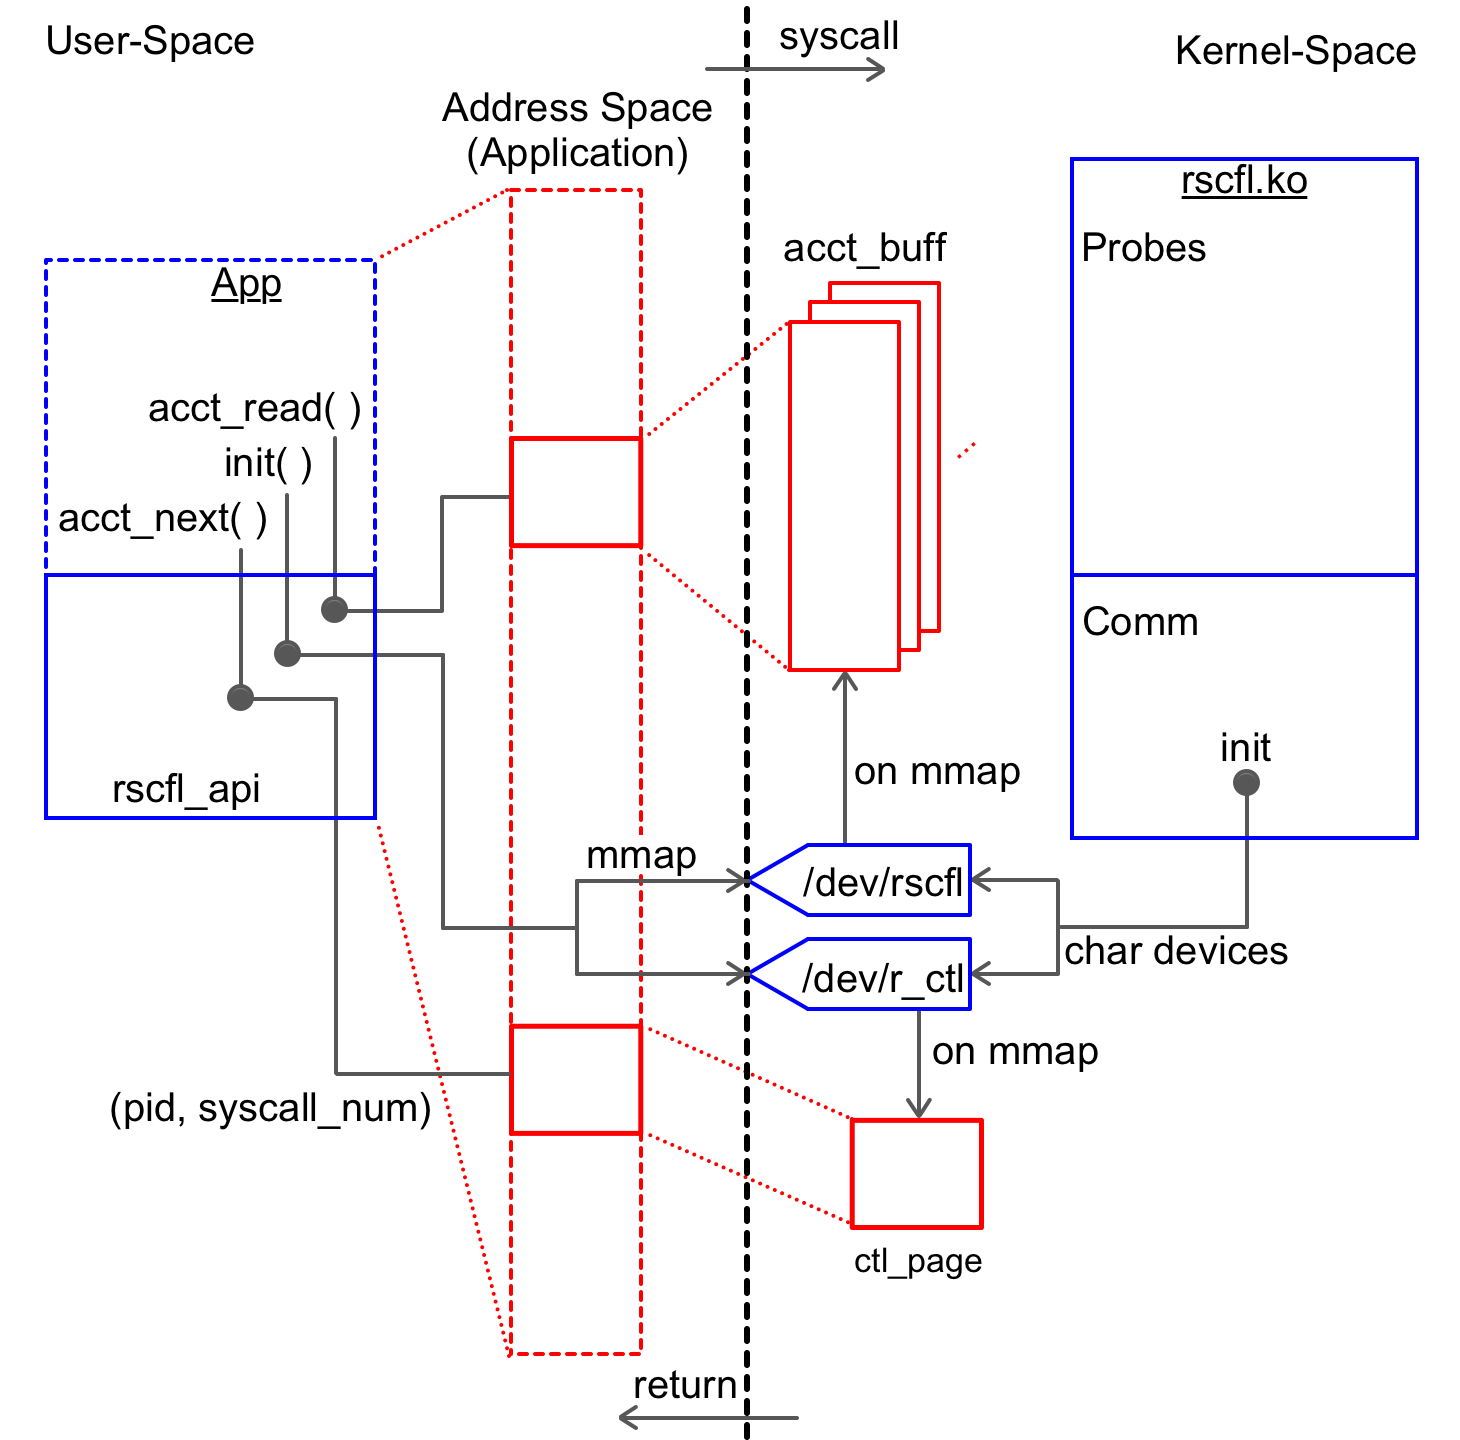
\includegraphics[width=0.7\columnwidth,natwidth=1460,natheight=1440]{sys_design}
	\caption{Primary user-space/kernel-space interactions detailed. Resource
accounting data is requested by applications for specific system calls and is
then available for reading (zero-copy) from kernel buffer regions mmap-ed into
the current address space. } 
	\label{fig:design}
\end{figure}

On initialization, the kernel module creates two character devices: a data
device (\texttt{/dev/rscfl}) for resource accounting information and a control
device (\texttt{/dev/r\_ctl}) for communication between user space and the
module. When applications linking with the \pname{ }library call
\texttt{init()}, the two devices are mmap-ed into their local address space. This
is done for each application thread, and the corresponding \texttt{mmap}
allocates a new buffer on the kernel side to hold resource accounting data for
system calls made from that thread.

On hitting a probe, the module needs to determine the corresponding accounting
buffer for writing resource consumption data. An index that links given
\texttt{pids} to their corresponding buffers is maintained in per-cpu hash
tables for this purpose, avoiding locks on the critical path. \pname{ }
intercepts calls to scheduler functions in order to maintain those indexes
up-to-date for each cpu.

\subsubsection*{Accounting for Asynchronous Resource Consumption}
As described in our initial example, the total cost of performing a buffered
write should also consider the asynchronous operation committing the data to
disk. Unlike existing approaches, \pname{} separately reports the resources
consumed asynchronously after making such system calls.  Without reporting the
amortized, asynchronous cost, current performance monitoring APIs provide an
incomplete representation of system resource consumption.

The solution for tracking calls that have caused a given asynchronous task
hinges on the observation that a link between two operations can only exist if
the kernel code maintains some data structure shared by both. \textit{Cache
buffers} in which data is enqueued and later dequeued asynchronously (flushed)
and \textit{timers} started by a function for running a given task when reaching
zero are just two examples. Tracking the lifetime of those shared structures and
any actions performed on them is sufficient for determining the calls to which
resource consumption should be attributed.

When multiple system calls are amortized over the same asynchronous operation
(e.g. multiple writes being buffered and then flushed to disk once),
the resources consumed by the flush will have to be divided amongst all the
initial system calls, following an \textit{attribution strategy}. For buffered writes,
the simplest strategy is to divide the costs proportional to the size of each
write.

\pname{ }performs accounting for asynchronous kernel operations by observing
that Linux provides a number of abstractions for performing asynchronous work:
\emph{timers}, \emph{tasklets}, \emph{workqueues} and \emph{interrupts}. Each of
these is characterized by particular shared data structures, and the framework
will index their addresses in order to track the operation that triggered the
asynchronous execution.

Custom asynchronous accounting can also be set up: Listing~\ref{lst:config}
shows how network scheduler buffers (the qdisc buffer) can be tracked across
enqueue/dequeue operations: when the \texttt{dev\_queue\_xmit} probe is hit
(synchronously), \pname{ }will store the address of the qdisc buffer. A
following \texttt{qdisc\_restart} probe being hit on an asynchronous path will
match on the address of the qdisc buffer and search the index for the correct
accounting structure that should be filled.

% Async / Sync tracing (multiple layers, kworkers etc).
%Call granularity tracing.
%Trace-point idenfitication - CScope, call site vs function.
%Moving from ST to KProbes (more dynamic).

\subsection{User space API}
The core of \pname{ }user's space API is formed by the three functions presented
in Figure~\ref{fig:design}. \texttt{init()} must be called by the application on
every thread that needs resource consumption data, and returns a handle used by
the other functions in identifying the locations of mmaped buffers. 

Before a system call of interest, the developer calls
\texttt{acct\_next()}. This will write an entry to the control device marking
the fact that the kernel infrastructure must track resource consumption for the
next system call comming from that \texttt{pid}. Variants of
\texttt{acct\_next} exist, in case the developer needs accounting for the next
\textit{n} system calls, or just needs to start/stop accounting at specific
points in the application. \texttt{acct\_next} also allows the user to pass in a
bit array in order to filter-out uninteresting kernel sub-systems from the
result. Custom aggregation can be set up by passing an integer token
(arbitrarily chosen by the user) to multiple \texttt{acct\_next} calls. The data
for all the calls with a given token value will be aggregated in the same
accounting structure.
%The same bit array will be updated to match the actual results when reading them.

The third API call, \texttt{acct\_read}, allows zero-copy reads of accounting
data from the kernel. Synchronous costs can be read immediately, and a callback
can be set up for running when the asynchronous part of the cost has also been
recorded. The returned data structure contains the same bit array used to apply
filters, but this now specifies which subsystems the system call has actually touched
(in this way, the application knows which elements of the structure contain valid data).

An API extension which we have not yet implemented in our prototype will allow applications
to \texttt{mmap} resource accounting buffers of other processes. This paves the way for applications that
react to concurrent workloads, by throttling or delaying their own
operations for example.

\section{Initial results}
We have developed the kernel subsystem identification and resource accounting
prototypes separately, with the purpose of showcasing the feasibility of the design
and gathering preliminary overhead data.

At the moment, the kernel module uses SystemTap to manually set kprobes for the
network, memory and filesystem kernel sub-systems.

In order to understand the overhead introduced by \pname, we have modified
\textit{lighttpd} to link with our user-space library and do resource accounting
for each socket accept/send/receive call. At runtime, lighttpd is configured to serve
a number of static files for performing end-to-end latency and throughput tests.

To characterize overhead, we first look at the distribution of latencies and
compare a vanilla lighttpd binary with the one that runs resource accounting
using \pname, for 10{\kern 0.12em}000 sequential requests issued using \texttt{http\_ping}. As
observed in Figure~\ref{fig:experiment1}, the median latency increases by 3.9\%
when resource accounting is active. The tail latency is also slightly increased,
with the 99th percentile growing by 7.66\%.
\begin{figure}[ht!] 
	\centering
	%\hspace*{-0.05\columnwidth} 
	\def\svgwidth{0.7\columnwidth}
	\input{overheads.eps_tex}
	%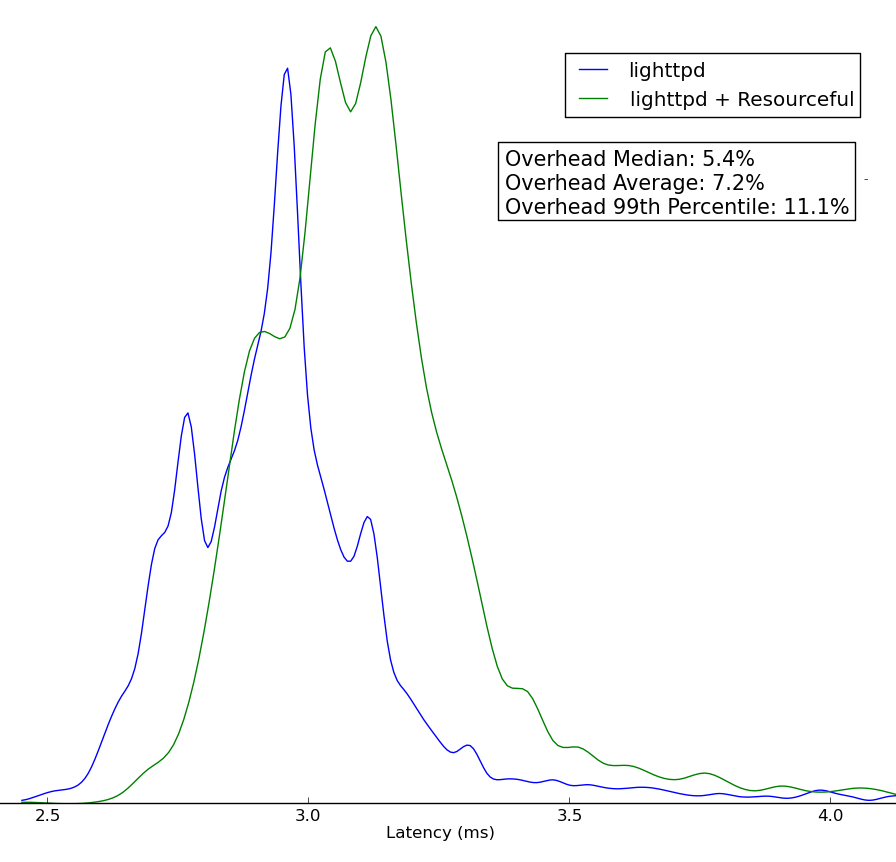
\includegraphics[width=1.1\columnwidth]{dist_and_fit2}
	\caption{Normalized latency histograms showing changes in latency distribution when enabling \pname{ }for lighttpd} 
	\label{fig:experiment1}
\end{figure}

Importantly, the overall characteristics of the latency distribution stay the
same: we see two local maxima and the overall shape remains similar. This
suggests that even with the overhead of measuring resource consumption, one
would still observe the latency characteristics of the underlying system. 

Table~\ref{fig:design} shows the drop in throughput ({\raise.17ex\hbox{$\scriptstyle\sim$}}31\%) averaged over 10
runs when doing 100k sequential requests for small files using \texttt{http\_load}. This should
be seen as an overhead upper-bound, as we have not yet performed any
optimizations on the system as a whole. An in-depth evaluation is planned as
future work.

\begin{table}[ht!]
	\centering 
    \begin{tabular}{|l|l|l|}
    \hline
    \textbf{lighttpd}         & Base & + \pname \\ \hline
    Fetches / second (avg) & 2486.4 & 1716.9 \\ \hline
    %Fetches / second (Min) & 2485.7 & 1711.5\\ \hline
    %Fetches / second (Max) & 2497.7 & 1721.7\\ \hline \hline
    Bytes / second (avg) & 54700.5 & 37772.0 \\ \hline
    %Bytes / second (Min) & 54685.7 & 37653.7 \\ \hline
    %Bytes / second (Max) & 54950.3 & 37876.4 \\ \hline
    \end{tabular}
    \caption{Change in throughput when enabling \pname{ } for lighttpd}
    \label{tbl:throughput} 
\end{table}

\section{Related work} 

%Existing tracing / profiling systems. (Maybe a chart
%outlining differences).

%FTrace, SystemTap (raw) / DTrace, Perf.

%Existing use of tracing for dependability.\newline Root-cause analysis.
%Debugging. Performance monitoring - how do we compare to top?

Many existing tracing and profiling tools only instrument a thin layer of the
target system. For example Dapper \cite{dapper} makes use of instruments in an
RPC library and X-Trace \cite{xtrace} modifies only the protocol and network
stacks. Whilst these tools are able to provide detailed information about their
respective instrumented layers, they treat much of surrounding system as a
black-box. The Google-Wide Profiling tool \cite{gwp} attempts to overcome this 
narrow view by profiling the entire target system, but instead of being continuous 
it is sample-based, meaning it makes a trade-off between sample rate and visibility. 
\pname{ } differs from these by allowing any part of a target system
to be continually profiled whilst only incurring a low-overhead.  

Other tracing systems such as Magpie \cite{magpieosdi} require the user to
provide a definition of the expected system structure in order for it to
correctly correlate events. \pname{} automatically identifies subsystem
boundaries, although those can also be manually configured by the user.

The primary method of interacting with \pname{} is through its user-space API.
Other systems such as Fay \cite{fay} go some way towards providing a programmatic
interface to trace and profile data, but are still limited to a post-hoc
evaluation. \pname{}'s API allows trace data to be retrieved and evaluated in
line with the target processes execution. This runtime availability of resource
consumption data give a much richer view of how the application and kernel are
performing, allowing for more informed decisions to be made. 

One useful feature to have when designing a dependable system is being able to
accurately predict the future. The system described by Ostrowski et al
\cite{ostrowski} provides methods for users to carry out what-if analysis on
existing trace data. \pname{} not only provides the primitives to build such a
system but allows the user to make decisions and take action at run-time when
provided with the results of a what-if scenario.

%something about the use of tracing and profiling in dependible systems

%systems left to talk about: Causeway, Racetrack, AJAX Scope, Triage, FALCON,
%X-Ray, GWP, Nirvana & iDNA

% NOTES(lc525): Weatherman is Ostrowski's work (already in)
% systems discussing multiple workloads interracting?

\section{Future work and conclusion} 
A number of challenges remain as future work: (i) evaluating the precision and
accuracy of the resulting data, thus characterizing the limits of our system -- this
would allow \pname{ }to be used for setting fine-grained quotas or diagnosing
software variability (ii) exploring whether some user-space instrumentation can
be automatically added using either compiler-based methods or binary rewriting.
(iii) extending \pname{ } to the hypervisor level and across hosts.

Measuring resource consumption at a fine-grained level is extremely useful in
understanding the behavior of a system and its interactions with the runtime
environment. However, the main problem with measurements like these is the
\emph{probe effect} they introduce. The main purpose of our developed prototype
is showing that it is feasible to obtain fine-grained accounting data without
significantly altering the characteristics of the system we measure (which, in
turn, means minimizing overhead). Longer term, we envision applications
coordinating their resource usage or even trading resources based on given
policies, using the same fine-grained accounting mechanisms.


{\footnotesize \bibliographystyle{acm} \bibliography{hotdep}}

\end{document}
